\chapter{Background Theory}
\label{background-theory}
Before we move to the nuts and bolts of AlphaZero and the concrete implementation for Abalone, we should establish a general understanding of the problem. That includes building the necessary theoretical background in artificial intelligence in general, as well as insight into specialized knowledge such as deep reinforcement learning in particular.

\section{Artificial Intelligence}
The introduction has already foreshadowed how artificial intelligence has undergone a shift in its methodology. In the 1950s and 1960s, figures like Alan Turing and von Neumann laid the foundations for modern computers. These new machines sparked the idea that one could create programs with similar abilities to humans and other organisms. Researchers at that time assumed there was no "universal principle" behind intelligence and focused on reason and symbol manipulation. Therefore these methods were considered "strong techniques," methods that relied on general principles like learning were labeled "weak techniques ." Nowadays, the consensus in the field has reversed. \cite[cf. p. 8f.]{sutton_reinforcement_2018}

% definition of artificial intelligence

\subsection{Rational Agent}
Any setting that involves artificial intelligence has an agent. Stemming from the Latin word \textit{agere} meaning "to act," an agent is something that acts. As one expects an agent to take sensible or intelligent actions, the definition must be further qualified by calling the agent rational. A rational agent acts "to achieve the best outcome or, when there is uncertainty, the best expected outcome." \cite[p. 36]{russell_artificial_2021}

The agent exists in an environment that it perceives through sensors and takes actions through its actuators. The content of the sensor's output for one observation is referred to as \textit{percept}: A cat uses eyes, ears and other organs to perceive the world and its legs, claws, and so on to interact with the world. An autonomous car might use radar and cameras for acquiring information and steering and motors for navigation.

Internally the agent might have some built-in knowledge about the world, such as rules on how the environment works. The \textit{agent function} takes the entire history of percepts observed and this built-in knowledge and maps it to an action. A concrete implementation of this abstract function is called \textit{agent program}. The agent program might just be a simple tabular mapping from percepts to actions or a complex algorithm with an additional model.

This abstract definition of an agent encompasses a simple program that plays Tic-Tac-Toe, but also very complex scenarios like a humanoid robot tasked to help in the household.

\subsection{(Task) Environment}
\label{environment}

As we are trying to build an agent that tries to achieve some specified goal, we can consider its environment as a problem or \textit{task} the agent tries to solve. The Tic-Tac-Toe program lives in a game world with simple rules while the humanoid robot has to interact with the physical reality. The environment might change either due to other influences or by the agent's actions. Putting together both agent and the environment, we see a loop of observing, deliberating, and finally taking an action as depicted in figure \ref{agent_environment_loop}.

\begin{figure}
    \centering
    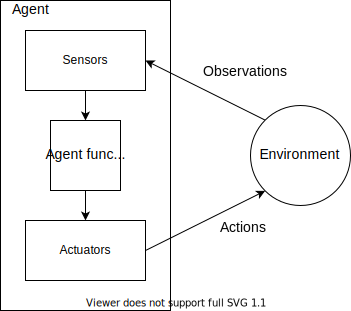
\includegraphics[height=7cm, keepaspectratio]{agent_environment_loop.png}
    \caption{The agent-environment interaction loop \cite[cf. p. 96]{russell_artificial_2021}}
    \label{agent_environment_loop}
\end{figure}

To specify the task environment, there are four core components illustrated for a machine classifying defective parts in a production line:

\begin{enumerate}
    \item Performance measure: This might be the percentage of correctly broken parts (true positives) weighed against the number of incorrectly identified parts (false positives).
    \item Environment: The conveyor belt and the parts
    \item Actuators: An arm to push the parts to a different conveyor belt
    \item Sensors: Possibly a camera, infrared sensors, etc.
\end{enumerate}

The initial letters form the acronym PEAS (framework). Aside from the specification of the task environment, there are also a few categorizations of the properties of task environments that are extremely helpful for narrowing down the potential applicability of different classes of algorithms.

A fundamental property is the observability of the environment. If the environment is \textit{fully observable}, the sensors detect all the information that is in any way relevant for taking an action. Conversely, if not all information can be observed, we call it \textit{partial observability}. For example, in poker, the other player's cards and the upcoming cards cannot be seen but are highly relevant to the agent's actions. As the current board state of chess entirely comprises all information necessary to make a move, we can classify it as fully observable.

The values of the state of the environment and time can be categorized into discrete and continuous. For instance, an autonomous vehicle deals with continuous time and continuous states. The car's speed takes a smooth range of real values, and time can be meaningfully split into increasingly small intervals. Board games are entirely discrete. The set of all states is a finite collection of all (legal) configurations of the board and the gaming pieces. Time progresses on the basis of turns.

An agent's actions might also be \textit{non-deterministic}. When dealing with systems of high complexity, the next state might not only depend on the previous state and the action taken. Other car drivers might take unexpected actions, or a comet hit the car.

Further expanding on the passage of time it has to be taken into account if actions have consequences for future states. If each combination of percept and action is independent of each other it is called \textit{episodic} and \textit{sequential} otherwise. If one had to classify a production line of circuit boards as either defective or functional, it would be an episodic environment. The classification of an individual board does not matter for the next one.

Another aspect of time is whether the environment changes while the agent takes time to deliberate on the next move. In a \textit{dynamic} environment like the autonomous vehicle operates in, the environment changes continuously. By the time the car decides whether to go right, to avoid collision with a wall, this decision might have already become obsolete. A  turn-based game like chess is static as the board only changes when a move is made.

Lastly, an additional dimension to consider is the number of agents involved. The classification of circuit boards only involves one agent whereas chess is a \textit{multi-agent} environment. We also have to distinguish whether those multiple agents compete for the performance measure. In most board games, one player's win is the other player's loss. In contrast, the other vehicles apart from our autonomous vehicle all profit when it avoids a collision and vice versa. Therefore, they cooperate.

\section{Adversarial Search}
With an intricate understanding of the environment of agents the choice of algorithms one can employ can be narrowed down. In general, perfect information games can be solved by adversarial search algorithms. That means in theory one can find the optimal solution by considering all legal moves and the resulting game states up until terminal states (game ending states). This is the \textit{game tree}. It contains all possible transitions between board positions (nodes) through moves (edges). The root of the tree is the default start position. The \textit{search tree} is potentially a subset of the game tree, if not all paths are visited or the search is not started at the starting position. The theory behind this type of algorithm was already laid out as early as 1945 by Konrad Zuse's program generating legal chess moves \cite{knuth_early_1980}, but was described most comprehensively by Claude Shannon in 1950 in "Programming a Computer for Playing Chess". \cite{shannon_xxii_1950}

\subsection{Minimax Algorithm}
Minimax assumes two roles: The minimizer ($min$) and the maximizer ($max$). The search starts from the current board state as the role of the maximizer and then alternates between the two. The result of the minimax search gives the maximum utility for the given state, assuming both players behave optimally. Let us define the functions \cite[p. 303f.]{russell_artificial_2021}
\begin{itemize}
    \item $\texttt{utility}(s, p)$ returns the utility or the payoff for the terminal state $s$ seen from the perspective of player $p$. In the case of chess this might be $-1, 0$ and $1$ for a loss, draw and a win.
    \item $\texttt{is-terminal}(s)$ returns whether the given state $s$ is a terminal state or not.
    \item $\texttt{to-move}(s)$ returns the current player for the state $s$, either $min$ or $max$.
    \item $\texttt{result}(s, a)$ returns the resulting state if in state $s$ and taking action $a$.
    \item $\texttt{actions}(s)$ returns all legal moves for the given state $s$.
\end{itemize}

\begin{equation}
    \texttt{minimax}(s) =
    \begin{cases}
        \texttt{utility}(s, max)                                                      & \texttt{is-terminal}(s)    \\
        \texttt{max}_{a\in\texttt{actions}(s)}\texttt{minimax}(\texttt{result}(s, a)) & \texttt{to-move}(s) == max \\
        \texttt{min}_{a\in\texttt{actions}(s)}\texttt{minimax}(\texttt{result}(s, a)) & \texttt{to-move}(s) == min \\
    \end{cases}
\end{equation}

Putting this together we can see in figure \ref{minimax} a graphical representation of the search tree for an abstract example. The algorithm traverses down to a leaf node, evaluates its utility and passes the value back up to the parent node. Depending on whether it is a minimizer or a maximizer it chooses the smallest or the largest value passed up by its children. This value again is passed up to the parent until the algorithm reaches the parent node which is always a maximizer, yielding the maximum utility the maximizer can achieve given the opponent plays optimally.

\begin{figure}
    \centering
    % \includesvg[height=7cm]{minimax.svg}
    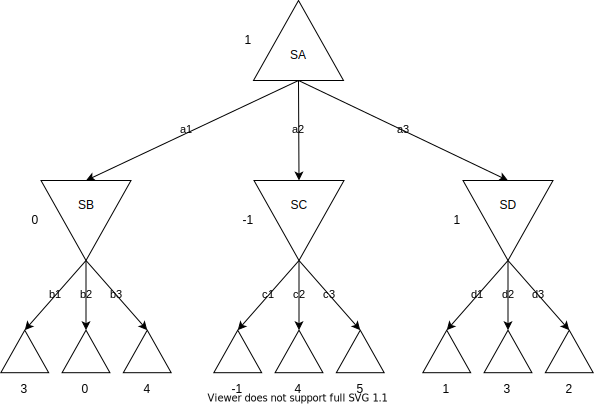
\includegraphics[height=7cm, keepaspectratio]{minimax.png}
    \caption{Minimax for a small search tree, resulting in an utility value of 1 \cite[cf. p. 303]{russell_artificial_2021}}
    \label{minimax}
\end{figure}

\subsection{Heuristic Functions}
As the number of nodes of the game tree gets very large, the search on the tree usually does not reach terminal leaves that indicate a clear loss or win. The computational resources will get exhausted first. For example minimax has already visited $ 361 * 360 * 359 * 358 = 16,702,719,120 $ nodes at a depth of $ d = 4 $ in the case of an average Go game.

Therefore, one has to limit the search to a computationally feasible depth and evaluate the intermediary result of a given transposition based on a so-called \textit{heuristic function}. This function replaces our previous $ utility(s) $ for terminal states and is based on human knowledge. The function should give precise feedback on the quality of a state from the perspective of the given player. Most commonly, the heuristic function combines multiple evaluations of a state into a total numerical value \cite[cf. p. 316]{russell_artificial_2021}. For instance in chess, the evaluations $ f_i $ could be be functions calculating different values such as:

\begin{itemize}
    \item Material: First, each piece is assigned an integer that represents the piece's relative value (pawn = 1, bishop/knight = 3, rook = 5, and queen = 9). Then sum the values of the pieces left on the board for each player.
    \item Space: Count the squares controlled by each player.
    \item King safety: Check weaknesses in king's position, count attacking pieces close to the king etc.
    \item Win and loss: As a more definitive measure to indicate whether the current state is a terminal state and hence a winning or losing state.
\end{itemize}

These evaluation functions can be combined into a linear combination of the form of:

\begin{equation}
    h(s) = \omega_0f_0(s) + ... + \omega_nf_n(s)
\end{equation}

By applying different weights $ \omega_i $ to the functions $ f_i $ the agent essentially is given an incentive to prioritize certain behavior. If the win or loss function returns a value of either $-1$ or $+1$, one might combine it with a weight of 10,000 to make sure we choose winning states and avoid losing states above all. Armed with this heuristic function one can find good moves with minimax search even in highly complex state spaces.

However, the problem with heuristic functions is that they require expert knowledge and a lot of empirical testing to find a suitable heuristic. In some cases like Go, such a heuristic function might not be competitive with even moderate human players. In other cases such as chess this strategy is very powerful. As mentioned in the introduction, IBM's Deep Blue could beat the world's best player Gary Kasparov with heuristic based adversarial search.

\subsection{Alpha-beta Pruning}
The minimax search can be improved markedly by using Alpha-beta-pruning. This method tries to eliminate unnecessary traversals down the search tree. In the best case, this leads to a reduction of nodes from $ O(b^d) $ to $ O(\sqrt{b^d}) $.

\begin{figure}
    \centering
    % \includesvg[height=7cm]{alpha_beta_pruning.svg}
    \includegraphics[height=7cm, keepaspectratio]{alpha_beta_pruning.png}
    \caption{The previous example but with alpha beta pruning applied. The grayed out nodes indicate, that these in fact could be pruned from the tree \cite[cf. p. 308]{russell_artificial_2021}}
    \label{alpha_beta_pruning}
\end{figure}

The order in which the nodes are visited in minimax is similar to a graph traversal with depth first search, meaning the algorithm descends down until it finds a leaf node. This gives information about the utility of that node and, consequently, part of the tree. Going up the tree an alpha value is kept for the minimum value the maximizer will receive and a beta value for the maximum value the minimizer will achieve. For instance this lets one know if the minimizer already can choose a move worse than what can be achieved with another move. The algorithm does not descend further $ (\alpha > \beta) $.

Looking at the example in figure \ref{alpha_beta_pruning} will help illustrate this principle. The search revealed that choosing move $ a_1 $ will yield a utility of at least $0$. Traversing down move $ a_2 $ the first leaf has a utility of $-1$. Hence, the minimizer will choose a move that is at most $-1$ which is already worse than the utility of $0$. One need not look further at this part of the tree.

The example also shows us an important prerequisite for this method to work. The order in which each node is expanded matters as it decides how many nodes we can prune. Had the algorithm visited move $ c_3 $ and $ c_2 $ first, pruning wouldn't have been possible. The best case of $ O(\sqrt{b^d}) $ is entirely dependent on this ordering. There are different ways of ranking the moves:

\begin{itemize}
    \item \textit{Killer move heuristic} prioritizes moves that are usually undoubtedly good like taking a piece in chess.
    \item \textit{Iterative deepening} Performs a minimax search only to a depth of one and uses the resulting values to rank the moves. Then searching one level deeper we use this ranking for ordering the moves. Even though there is a lot of redundancy, it is made up for more than enough by pruning much more effectively.
\end{itemize}

Other improvements to the procedure are thinkable as well. Once one performs a search for a certain state, the resulting utility can be stored. If this position is encountered again, because of a different move sequence (transposition), the state's utility can be looked up in the \textit{transposition table}.

Combined with alpha beta pruning, the minimax algorithm is a very efficient way of finding the optimal utility in an adversarial search situation. However, as mentioned before, in most games the utility of the terminal states cannot be used, because the search tree grows too quickly. By optimizing for a heuristic function the quality of play solely depends on this function. For games such as chess minimax has been very successful, because humans could devise meaningful heuristic functions. The chess engine stockfish has been the most successful computer player for a long time and is based on this algorithm (and many optimizations). \cite{noauthor_stockfish_2021, noauthor_stockfish_nodate}

\subsection{Monte Carlo Tree Search}
For games like Go it was deemed impossible to find powerful heuristic functions, which makes the previous approach of minimax not a viable option. In addition, the initial position of a $19 \cdot 19$ Go board has a branching factor of $361$ decreasing only by one for each stone placed. A method proposed in 2006 by Coulom \cite{coulom_efficient_2007} called Monte Carlo Tree search was more successful for Go. The main idea is to use simulations or \textit{rollouts (or playouts)} to gain information on the quality of a state. To manage the complexity of the search tree more effectively the algorithm is \textit{selective} in which parts of the tree are \textit{expanded}. This ensures that resources are not wasted on unpromising moves.

In its purest form the simulations are performed randomly.This means for a state or node to be investigated, two random players take turns until a terminal state is reached. Kocsis and Szepesvári \cite{kocsis_bandit_2006} showed that it does in fact converge to optimal play. For games with a high branching factor a large number of simulations is needed to get any meaningful information from the simulations. Hence a non-random \textit{rollout policy} could be used instead. The policy may guide the moves taken in the simulation towards better moves. This might be as simple as favoring capturing moves or as we will see later neural networks.

The algorithm iteratively expands the search tree. For each iteration it runs through four steps:
\begin{itemize}
    \item \textbf{Selection} is the process of deciding which node to consider next. Starting at the root node a node is selected until a leaf node is reached. This is the selected node. The selection of the nodes could be based on some probability distribution or use the knowledge gained over time.

    \item \textbf{Expansion} is the step in which the selected node is expanded by appending a fresh child node.

    \item \textbf{Simulation} is as described before the step in which a a simulation is performed with a rollout policy starting from the state of the newly generated child node.We take t

    \item \textbf{Back-propagation} is the last step. The result of the simulation (utility) is taken and written to the node and parent nodes above until the root node is reached. Each node updates its cumulative utility $U(n)$ and the number of times it was visited $N(n)$. It is important to note, that this to be differentiated from backpropagation in the context of neural networks (c.f. \ref{neural_networks}).
\end{itemize}

The more this cycle is repeated, the more certainty is gained about the best move to take.

\begin{figure}
    \centering
    % \includesvg[height=7cm]{minimax.svg}
    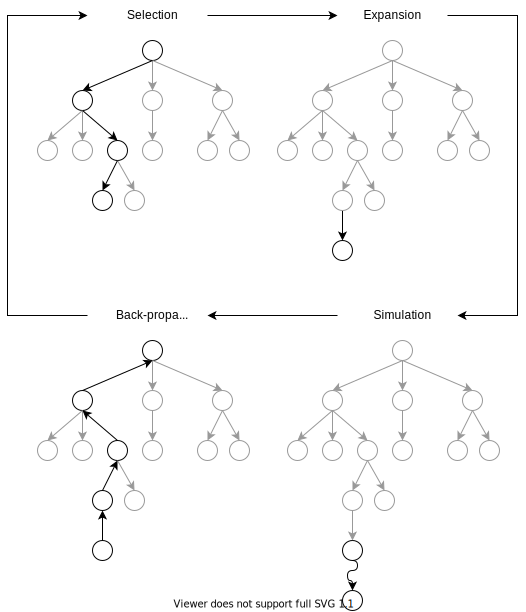
\includegraphics[height=9cm, keepaspectratio]{monte_carlo_tree_search.png}
    \caption{Monte Carlo tree search stages, cf. \cite{noauthor_fig_nodate}}
    \label{monte_carlo_tree_search}
\end{figure}

The development of MCTS led to significant improvements in performance of game-playing agents in the game of Go. The algorithm "Crazy Stone" from Coulom won the 10th KGS computer-Go tournament against competitors such as Indigo \cite{bouzy_associating_2006}. In the selection phase Crazy Stone estimates the probability of that move being better than the current best move and selects them according to that probability. The probability distribution over the moves is similar to the Gaussian distribution and the Boltzman equations. \cite[p. 4]{coulom_efficient_2007}

Another idea for selection is the upper confidence bound formula (\textit{UCB1}) \cite{auer_finite-time_nodate}, that weighs a node $n$ is visited and how promising it is. Let us define \cite[cf. p. 328]{russell_artificial_2021}:

\begin{enumerate}
    \item $\texttt{Parent}(n)$ returns the parent node of node $n$.
    \item $N(n) $ returns the number of playouts performed on node $n$ and its children.
    \item $U(n) $ returns the cumulative utility of node $n$. For instance, this might be the number of wins for node $n$ and its children.
\end{enumerate}

\begin{equation}
    \textit{UCB1}(n) = \frac{U(n)}{N(n)} + C \cdot \sqrt{\frac{\log{N(\texttt{Parent}(n))}}{N(n)}}
    \label{eq:UCB1}
\end{equation}

The cumulative utility $U(n)$ is normalized by the number of times the node was visited $N(u)$. This helps favor moves that are either relatively unexplored and promising or have proven to be good over a larger set of nodes. It is also called the exploitation term. The additional term is called the exploration term. The more often a node is visited, the smaller this term gets, converging to $0$ for large $N(n)$. The constant factor $C$ is subject to some debate which value might be optimal, some choose $\sqrt{2}$. In general, this hints at another point of investigation: The problem of \textit{exploration vs. exploitation} \ref{exploration_vs_exploitation} that we will inspect more closely later.

The leading researcher behind AlphaGo and AlphaZero, David Silver, started his research on Go with MCTS. As early as 2006 he, and Sylvian Gelly, investigated optimizations to MCTS \cite{gelly_achieving_nodate} for the game of Go. In 2011 they published a comprehensive paper \cite{gelly_monte-carlo_2011} proposing the algorithm MoGo and evaluating different strategies to improve the effectiveness of MCTS in Go. Seeing that

\begin{quotation}
    [...] professional Go players often play moves according to intuitive feelings that are hard to express or quantify. Precisely encoding their knowledge into machine-understandable rules has proven to be a dead-end: a classic example of the knowledge acquisition bottleneck. \cite[p. 1873]{gelly_monte-carlo_2011}
\end{quotation}

One of the ideas introduced is Rapid Action Value Estimation (RAVE). It was already mentioned how one could reuse information gathered for minimax through a transposition table. In a search tree one will encounter transpositions for that searches were already performed. RAVE allows to reuse experience gathered from simulations for related positions. A key property observed by Silver was that MoGo scales proportional to the amount of compute or rather number of simulations it can perform per turn as depicted in figure \ref{mogo_scaling}.

\begin{figure}
    \centering
    \includegraphics[height=7cm, keepaspectratio]{mogo_scaling.png}
    \caption{Elo rating of MoGo in relation to the computational resources granted to the algorithm \cite[p. 1872]{gelly_monte-carlo_2011}}
    \label{mogo_scaling}
\end{figure}

\section{Reinforcement Learning}
The methods described until this point can be described as "Good old fashioned AI". They rely on search and human knowledge to perform adequately. Now we shift our focus to methods that use learning mechanisms to improve their play. With MCTS we've actually seen a kind of intermediary form of algorithm as it is "simulating moves into the future, observing the outcome, and using the outcome to determine which moves are good ones is one kind of reinforcement learning." \cite[p. 331]{russell_artificial_2021}

By devising a heuristic function, we basically told our agent what to do by indicating how a good position looks. The agent optimized its actions to be in a good position as described by the function. In reinforcement learning the agent learns what action to take through interaction. We don't predefine which actions are to be taken. The agent tries to discover which actions yield the best \textit{reward}. The numerical reward signal might come immediately, but e.g. in the case of chess the reward for actions taken comes much later by winning the game (or losing it). According to Sutton and Barto those are the key components of reinforcement learning: "trial-and-error search and delayed reward". \cite[p. 1]{sutton_reinforcement_2018}

Reinforcement learning is not a specific solution or method, all methods for "goal-directed agents interacting in an uncertain environment" \cite[p. 3]{sutton_reinforcement_2018} are types of reinforcement learning. It is a general formalism that will help us reframe the problem of playing a board game (well) in a new light.

\subsection{Markov Decision Processes}
Central to reinforcement learning is a formalism for the environment called Markov decision process (MDP). The MDP introduces some constraints and specifications that are useful for making precise statements and building further theory on it. If the constraints and properties of a MDP apply to an environment, one can resort to the algorithms and proofs already built on the basis of MDPs. At the same time the constraints are so loose, that many learning problems can be formulated as MDP.

Basis for the MDP is the Markov Chain. Markov Chains are used to describe sequential decision making. Each decision results in a state. The transition between states is stochastic, which means the following state depends on a probability. The transition probability does not depend on the history of previous states, it is independent.

Richard bellman extended Markov Chains by actions and rewards to derive MDPs \cite{yang_markov_2019, bellman_markovian_1957}. Actions cause transitions between states. They have long-term consequences, thus, effect future reward. The passage of time is divided into discrete time steps $ t $ at which the agent senses the state $ S_t \in \mathcal{S} $ and then selects some action $ A_t \in \mathcal{A}(S_t) $. Resulting in that action is some reward $ R_{t+1} \in \mathcal{R} \subset \mathbb{R} $ that is received in the next timestep. This is very similar to the interaction loop previously discussed in figure \ref{agent_environment_loop}. We can reframe this image with the new terminology of the MDP framework in figure \ref{mdp_agent_environment}.

\begin{figure}
    \centering
    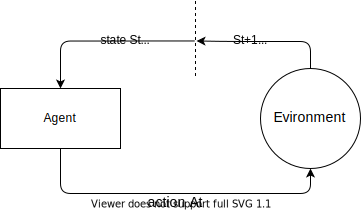
\includegraphics[height=4cm, keepaspectratio]{mdp_agent_environment.png}
    \caption{The markov decision process as agent-environment interaction loop \cite[cf. p. 48]{sutton_reinforcement_2018}}
    \label{mdp_agent_environment}
\end{figure}

For a \textit{finite} MDP the sets of all actions $ \mathcal{A}$ (\textit{action space}), states $\mathcal{S}$ (\textit{state space}) and rewards $ \mathcal{R} $ have a finite amount of elements. The transition probabilities between the state $ s $ and the next state $ s' $ and its reward $r \in \mathcal{R}$ is given by the function $ p $ which essentially defines the decision process as a whole. A game of chess is deterministic, all transitions have a probability of $1$ and these probabilities are defined by the rules of the game. However, the MDP is formulated to incorporate stochastic environments as well:

\begin{equation}
    p(s', r | s, a) = P\{S_t=s', R_t = r | S_{t-1} = s, A_{t-1}=a\}
\end{equation}

In a MDP, just as in a Markov Chain, "the state must include information about all aspects of the past agent environment interaction that make a difference for the future. If it does, then the state is said to have the \textit{Markov property}". \cite[p. 48]{sutton_reinforcement_2018} This means the transition probability $p$ is independent of the history of preceding states.

From these properties of the MDP we can define the four central components of Reinforcement learning:

\begin{itemize}
    \item \textbf{The reward signal} is the description of the agent's goal. A controller of a cooling system for a server farm might have the goal to minimize the energy spent for cooling while keeping the servers below a certain threshold. The reward signal then encompasses both of these subgoals. The controller has to maximize this reward. The \textit{reward hypothesis} states that:
          \begin{quotation}
              That all of what we mean by goals and purposes can be well thought of as the maximization of the expected value of the cumulative sum of a received scalar signal (called reward). \cite[p. 52]{sutton_reinforcement_2018}
          \end{quotation}
          Therefore, we introduce the reward $R_t $ and the goal $ G_t $ which is in the simplest case the sum of future rewards until the final time step $T$.

          \begin{equation}
              G_t = R_{t+1} + R_{t+2} + ... + R_T
          \end{equation}

          We might also discount the future rewards by some factor $\gamma \in [0, 1] $ to account for the decrease in certainty we have about future rewards:

          \begin{equation}
              G_t = R_{t+1} + \gamma R_{t+2} + \gamma^2 R_{t+3} + ... = \sum_{k=0}^{\infty} \gamma^kR_{t+k+1}
          \end{equation}

    \item \textbf{The policy} is a mapping between the perceived states to probabilities of selecting each possible action. For TicTacToe we might imagine a table that lists for all possible states to the agent's action. Due to the size of the state space \ref{complexity_table} in more complex games this would not be feasible, therefore we used search processes as a policy so far.

          We denote the policy as the function $\pi $. It defines a probability distribution over all actions $ a \in \mathcal{A}(s)$ for each $ s \in \mathcal{S} $. $ \pi(a|s)$ is probability at a given timestep $t$ for the action to be $ a = A_t $ under the condition that $ s = S_t $.

    \item \textbf{The value function} is an estimation of the reward for the agent to be in a given state $ s $. In other words, it is the expected value $\mathbb{E}$  for the goal $G_t$ given the state $s$. As the reward for a state depends on what actions we take in the future, the value depends on the policy $ \pi $ defined above. Given that we are at timestep $ t $ and in state $ s = S_t $, the \textit{state-value function $v_{\pi}$}:

          \begin{equation}
              v_{\pi}(s) = \mathbb{E}_{\pi}[G_t | S_t = s] = \mathbb{E}_{\pi}\left[\sum_{k=0}^{\infty} \gamma^kR_{t+k+1} \middle| S_t = s \right]
          \end{equation}

          The heuristic function encountered previously was essentially a value function being used to guide the game-tree search.

          Furthermore, we define the value of action $a$ while being in state $s$ under the policy $\pi$ as the \textit{action-value function} $q$:

          \begin{equation}
              q_{\pi}(s) = \mathbb{E}_{\pi}[G_t | S_t = s, A_t = a] = \mathbb{E}_{\pi}\left[\sum_{k=0}^{\infty} \gamma^kR_{t+k+1} \middle| S_t = s, A_t = a \right]
          \end{equation}

          \begin{figure}
              \centering
              \includegraphics[height=2cm, keepaspectratio]{policy_value_action_value.png}
              \caption{A visual explanation of policy, value and action-value \cite[p. 62]{sutton_reinforcement_2018}}
              \label{policy_value_action_value}
          \end{figure}

          The figure \ref{policy_value_action_value} shows how the three elements of policy, state-value and action-value relate to each other.

    \item \textbf{The model} helps to make predictions about how the environment might behave. For a given state and action it might return to the next state which aides in planning ahead. In the case of Abalone the model is the rules of the game, used by the function that returns all legal moves or the resulting board from a given board and a move.
\end{itemize}

The goal of reinforcement learning is to find (or approximate) a policy that maximizes the future reward for each action and state. For MDPs we define the \textit{optimal policy} $\pi_*$ as having higher or equal return than all other policies. Thus, the optimal policy maximizes the value function, resulting in the \textit{optimal state-value function}:

\begin{equation}
    v_{*}(s) = \max_{\pi} v_{\pi}(s)
\end{equation}

for all $s \in \mathcal{S}$. For instance, in chess the goal is to find a policy that approximates the utility returned by exhaustive search. Given such a policy one could evaluate the best possible outcome for any state $s$ with the optimal state-value function.

An example will help illustrate these abstract specifications. We might view a pick-and-place robot arm through the lens of reinforcement learning. It has the task to place items from a pick-up location into a target area, cf. \cite{noauthor_examples_nodate}.

\begin{itemize}
    \item The state space $ \mathcal{S} $ is all possible combinations of the joint angles and velocities.
    \item The action space $ \mathcal{A} $ is the amount of voltage that can be applied to each of the motors.
    \item The rewards $ \mathcal{R} $ are $+100$ for each sucessfully placed item and a $-1$ reward is occurred each time a unit of energy is spent.
    \item Lastly, the state transitions $p(s', r | s, a)$ might be stochastic. The motors might have some imprecisions. An applied voltage might not always change the angle of a joint as expected.
\end{itemize}

In this scenario, the optimal policy $ \pi_* $ is to place the objects successfully with minimal energy expenditure. As mentioned in the introduction \ref{introduction}, researchers have sucessfully used RL methods to let robot arms learn, through interaction, how to pick and place items. The fundamentals described in this chapter are taken from \cite[p. 47ff.]{sutton_reinforcement_2018}, which goes more into detail about the details of MDPs and provides many additional examples.

\subsection{Exploration vs. Exploitation}
\label{exploration_vs_exploitation}
As the agent builds its knowledge while it is engaged in the environment it has to weigh \textit{exploiting} the gathered knowledge for ensuring a safe short term reward or sacrificing it for \textit{exploring} other actions that might turn out to bring higher rewards in the future. To illustrate this fundamental tradeoff in reinforcement learning, let us imagine a gambling machine with 10 levers, a 10-armed bandit. At each timestep $ t $ we have to decide which lever to pull and then we receive some reward $ R_t $. Each lever has some unchanging (\textit{stationary}) distribution over the rewards that is hidden from us. The distribution looks like the one given in figure \ref{10_armed_bandit}.

\begin{figure}
    \centering
    \includegraphics[height=7cm, keepaspectratio]{10_armed_bandit.png}
    \caption{The reward distributions of a 10-armed bandit \cite[p. 28]{sutton_reinforcement_2018}}
    \label{10_armed_bandit}
\end{figure}

To estimate the action-value of each lever, we sum the rewards received for that lever $ \texttt{total-reward}(a) $ and divide it by the number of times we've chosen the lever $ N_t(a) $ at the timestep $ t $.

$$
    Q_t(a) = \frac{\texttt{total-reward}(a)}{N_t(a)}
$$

This is called the \textit{sample-average} method. The simplest policy would be to just always choose the action with the largest sample-average $ Q_t $ a \textit{greedy} policy.

$$
    A_t = \operatorname*{argmax}_a Q_t(a)
$$

First all action-values $Q_t(a)$ are initialized with the value $0$.Initially, we might choose a random lever and that yields a reward of $0$. As all $ Q_t $ are still $0$ we choose another random lever giving us a reward of 1. Then, according to the greedy policy, we just repeatedly pull this lever indefinitely. The lever has the maximum action-value. We just get stuck on exploiting the small knowledge we have gained. To allow for some exploration of other actions. we introduce a small probability $\varepsilon $ of choosing a different (random) action: With a probability of $ 1- \varepsilon $ the agent chooses the greedy action, with a probability $ \varepsilon $ a different action.

If we continue for an infinite number of times the sample average for each action is guaranteed to converge to $ q_{*} $. Each action is sampled enough to estimate its stationary distribution. We might also let the $ \epsilon $ decay over time to ensure we exploit the optimal lever eventually. This shows how we have to carefully consider what knowledge we have and how we plan to expand it further. This also indicates the difficulty that is introduced when the problem is not stationary, which creates the necessity of continuous exploration.

\section{Deep Reinforcement Learning}
As reinforcement learning is a very general framework things like the value function $ v(s)$ are just left as an abstract function. There are many different methods that build on the foundation of MDPs and fill these abstract functions with concrete instructions. One such method is deep RL, where the RL is combined with deep neural networks. Deep neural networks are \textit{general function approximators}. Hence, they could be used to approximate the optimal value function $ v_{*}(s) $ to maximize rewards.

\subsection{(Deep) Neural Networks}
\label{neural_networks}

Neural networks are one specific machine learning method that has had large success in the recent past. Machine learning has been a paradigm shift in the way we think about building programs. In the classical development one uses the data and predefined rules as input for the development. This means we have to have intricate knowledge about the problem domain to produce the answers we want. For tasks like image classification this is a difficult process as it is very hard to think of patterns and conditions an image has to have, to find cats in them.

\begin{figure}
    \centering
    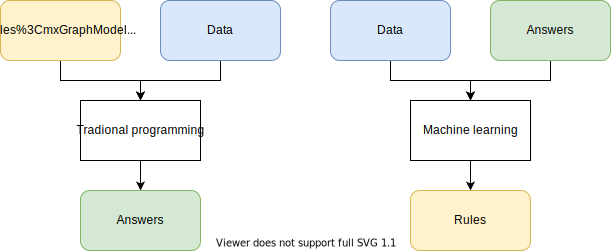
\includegraphics[height=5cm, keepaspectratio]{programming_paradigm_shift.png}
    \caption{A fundamental shift in how we think about programming \cite[cf. p. 5f.]{moroney_ai_2020}}
    \label{programming_paradigm_shift}
\end{figure}

In machine learning we use the answers and the data as input to the development process and the rules are the output we produce. Figure \ref{programming_paradigm_shift} contrasts this change in programming.

\begin{figure}
    \centering
    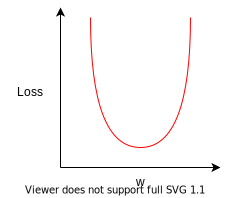
\includegraphics[height=5cm, keepaspectratio]{loss_curve.png}
    \caption{(a) Data points of price versus floor space of houses for sale in Berkeley, CA, in July 2009, along with the linear function hypothesis that minimizes squared-error loss: y = 0.232x + 246. (b) Plot of the loss function for various values of $ w_0 $, $ w_1 $. Note that the loss function is convex, with a single global minimum. \cite[p. 1251]{russell_artificial_2021}}
    \label{loss_curve}
\end{figure}

Consider any linear function of the form:
$$
    f(x) = w_1x + w_0,
$$
with $ x, w_1, w_0 \in \mathbb{R} $. We could use this function to make predictions about one dimensional input data. For example we might have a (training) dataset of living space of houses in $ m^2 $ $ X $ and their corresponding price $ Y $. Each row $X_i$ corresponds to the row $Y_i$. We could choose the bias $ w_0 $ and the \textit{weight} $ w_1 $ such that the squared error for all rows $i$ is minimal in a process we know as linear regression. When given new data our linear model can make predictions of the potential prices of the houses as described in figure \ref{loss_curve}.


\begin{figure}
    \centering
    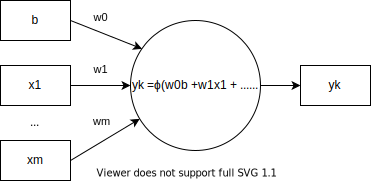
\includegraphics[height=4cm, keepaspectratio]{neural_networks.png}
    \caption{The fundamental idea behind neurons}
    \label{neural_network}
\end{figure}

\begin{figure}
    \centering
    \includegraphics[height=3cm, keepaspectratio]{neural_network_layers.png}
    \caption{A small neural network arranged in layers. An input layer, a hidden layer and an output layer}
    \label{neural_network_layers}
\end{figure}

\paragraph{Activation function}
An important component is not only the linear function but also the activation function: Before we pass the value of the function f(x) on, we apply some function $ \phi $. An activation function applied to a linear function is referred to as \textit{neuron}. The activation function allows us to introduce a non-linearity, which in turn makes smaller networks of neurons able to perform much better on more complex tasks than just a simple linear activation. Common functions used are:
\begin{itemize}
    \item ReLU: $ \phi : max(0, f(x)) $
    \item Sigmoid: $ \phi : \frac{1}{1 + e^{f(x)}} $
    \item Binary step: $ \phi : \begin{cases}
                  0 & f(x) < 0    \\
                  1 & f(x) \geq 0 \\
              \end{cases}$
\end{itemize}

This resulting basic neuron is depicted in figure \ref{neural_network}. If we want to make more complex inferences than just the prices of houses, we can arrange multiple neurons into larger structures like chains or layers (\ref{neural_network_layers}). To build such networks we need to generalize the linear function of the neuron for higher dimensional input:

\begin{equation}
    y_k = \phi\left(\sum_{j=0}^{m}w_jx_j\right)
\end{equation}

But this poses a problem. We can find globally optimal solutions for linear neurons with linear regression. However, this does not work for other activation functions. Moreover, as the size of the network grows, the computational cost of these methods grows too large. Moreover A different approach is necessary.

\paragraph{Loss functions} In the context of linear regression the term \textit{mean squared error} was already mentioned. It is the average squared difference between the predictions and the desired output:

\begin{equation}
    MSE = \frac{1}{n} \sum_{i = 1}^{n}(X_i - Y_i)^2
\end{equation}

This is one type of \textit{loss function}, which in general is a measure to describe the error we seek to \textit{minimize} in an optimization process.


\paragraph{(Stochastic) gradient descent and backpropagation} By utilizing the loss function we can feed an input into the network and measure for any permutation of the weights $ w_i $ how big the error of the network is. By measuring the loss of the training set $ X $ we can find out how well the current configuration of the network fits the data.

Let's go back to the problem of house price prediction. If we plot the MSE for the weights $ w_0 $ and $ w_1 $ of our single neuron the result is a parabola in figure \ref{loss_curve}. Ideally, we want to walk down into the valley where the error is minimal. So for any given combination of the weights we have to find out in which direction the downward slope maximal. The direction of the greatest change of a scalar function is called gradient, which is formalized as follows:

$$
    \nabla f(p)=\left[\begin{array}{c}
            \dfrac{\partial f}{\partial x_1}(p) \\
            \dfrac{\partial f}{\partial x_2}(p) \\
            \vdots                              \\
            \dfrac{\partial f}{\partial x_n}(p)
        \end{array}\right]
$$,
where the point $p $ is a point in the \textit{parameter space}, e.g. as depicted in figure \ref{loss_curve}(b) for $w_0 $ and $ w_1 $. For a single neuron we can use the methods learned in calculus to find the respective \textit{partial derivatives} $  \dfrac{\partial f}{\partial x_i}(p) $. By repeatedly calculating the gradient and updating the weights to move further in the direction of the downward slope, we describe the algorithm of gradient descent:

\begin{algorithm}
    \caption{Gradient descent outline \cite[p. 1253]{russell_artificial_2021}}\label{alg:gradient_descent}
    \begin{algorithmic}
        \State $w \gets \text{any point in the parameter space}$
        \While{not converged}
        \ForEach{$w_i$ in $w$}
        \State $w_i \gets w_i - \alpha \dfrac{\partial f}{\partial w_i}(Loss(w))$
        \EndFor
        \EndWhile
    \end{algorithmic}
\end{algorithm}

The variable $ \alpha $ for gradient descent describes the \textit{learning rate}, so by how much we update the weights. As we have to differentiate not only a single neuron but a network of neurons, some constraints have to be defined to make derivation possible:

\begin{itemize}
    \item All functions utilized by the neuron and the network (activation, linear combination of weights) have to be differentiable
    \item The network has to be a directed acyclic graph, thus, no loops etc.
\end{itemize}

This makes the neural networks one type of \textit{computational graph}, which have the convenient property letting us find the gradients of the weights in respect to the loss by \textit{backpropagation} by essentially applying the chain rule. Figure \ref{computational_graph} shows an example of a computational graph and its derivation.

\begin{figure}[!h]
    \centering
    \subfloat[Functions are nodes]{
        \includegraphics[width=6cm, keepaspectratio]{computational_graph_functions.png}
    }
    % \hfill
    \subfloat[Differentiate the graph by node $e$]{
        \includegraphics[width=6cm, keepaspectratio]{computational_graph_derivative.png}
    }
    \caption{An example of a computational graph \cite{colah_calculus_nodate}}
    \label{computational_graph}
\end{figure}

In summary, the neural network architecture describes a space of possible functions (or programs). The training data describes the desired output of the function. The loss function measures how much the output of the current configuration of the neural network differs from the desired output. Gradient descent adjusts the weights of the network in such a way that the ouput of the network fits the training data better: Gradient descent searches this space of functions for one that minimizes the error. Due to the nature of gradient descent, we are not guaranteed to find the globally optimal program. A different architecture might define a function space that contains more suitable functions than others.

\subsection{Convolutional Neural Network}
\begin{figure}
    \centering
    \includegraphics[width=\textwidth, keepaspectratio]{typical_cnn.png}
    \caption{A typical CNN architecture \cite{noauthor_convolutional_2022}}
    \label{typical_cnn}
\end{figure}

As already stated, the neural network or computational graph is not limited to one specific type of function as long as the function can be differentiated. As shown in \ref{neural_network_layers} in its basic form, neural networks have a $n$-dimensional vector as input. If we have an input like an image, we would have to break down the information about the adjacency to fit the form of a vector.

Furthermore, the computational requirements for such an approach would grow rapidly. A fully connected first layer would need $n^2$ weights for an image of the size $n$. A small image of the size $ 256 \cdot 256$ would need $65,536$ weights for the first layer alone.

To achieve this we can utilize convolution. In general terms a "convolution is an integral that expresses the amount of overlap of one function $g$ as it is shifted over another function $f$." \cite{weisstein_convolution_nodate}

$$
    (f * g)(x) = \int_{-\infty}^{\infty} f(t)g(x - t) dt
$$

This might seem very abstract but firstly, only the discrete case is relevant to us and secondly, only the finite case. This boils down the convolution to filtering $F$, which also comes up in image processing (technically this is the cross-correlation):

$$
    F(u, v) = \sum_{x} \sum_{y} I(u+x, v+y)H(x, y)
$$

\begin{figure}
    \centering
    \includegraphics[height=5cm, keepaspectratio]{convolution.png}
    \caption{Convolution of a 8x8 black and white image with a 3x3 kernel, no padding and a stride of 1. \cite[cf. p. 13]{bruasdal_deep_2020}}
    \label{convolution}
\end{figure}

For a given coordinate $u,v$ each value in the matrix $H$ (also called \textit{kernel}) is multiplied by the  corresponding value of the image returned by function $I$. The figure \ref{convolution} illustrates how a convolution would look on a black and white image. In image processing for example, we might use a Laplacian filter to extract certain features like edges. By using convolutions in a neural network we move away from these hand-crafted features by letting the parameters of the kernels be trained to fit the desired outcome. The result is a \textit{convolutional neural network} (CNN) as depicted in figure \ref{typical_cnn}. The properties (and advantages) of CNNs are:

\begin{itemize}
    \item By combining multiple layers of convolutions the network can extract higher level abstractions of the image \cite{ilin_abstraction_2017}. This also introduces sparsity between the layers, as a neuron is only connected to a part of the previous layer.
    \item The output of the network is equivariant to translation. This means that a pattern found in the corner produces the same magnitude of a response as a pattern found in the center of the image. However, the response is in a different location. \cite{208949}.
\end{itemize}

The application of this method for image related tasks has become very popular. The first large scale application in 2012 by Krizhevsky et al. \cite{krizhevsky_imagenet_2017} vastly outperformed any previous methods. This approach is very relevant to the board game setting in Abalone as each board position is essentially an image. Patterns of marbles are relevant in different positions of the board just as different shapes and objects in different places in an image.

\subsection{Residual Networks}
By stacking many layers a network can fit more complex domains. Their size has earned them the name \textit{deep neural networks}. But a central issue with increasing the size of the network is the problem of \textit{vanishing gradients}. For example, as the arguments approach $-\infty$ and $\infty$, the sigmoid function is in it's limit $0$ and $1$ respectively. The derivative approaches $0$ for both cases as depicted in figure \ref{residual_network} (a). That means in backpropagation, larger input values produce very small output values when passed through such a neuron. As the derivatives are multiplied during the backpropagation (chain rule) they become even smaller, thus vanishing as they further approach $0$ with each added layer.

\begin{figure}[!h]
    \centering
    \subfloat[Sigmoid function and its derivative \cite{noauthor_wolframalpha_nodate}]{
        \includegraphics[height=4cm, keepaspectratio]{sigmoid_vs_derivative.png}
    }
    % \hfill
    \subfloat[A residual block \cite{he_deep_2016}]{
        \includegraphics[height=4cm, keepaspectratio]{residual_block.png}
    }
    \caption{Motivation and implementation of residual networks}
    \label{residual_network}
\end{figure}

To mitigate this issue one could use different activation functions like the ReLU or use \textit{residual connections}. In a residual (or skip) connection the value of the input before passing through the neuron is added with some weight to the output as shown in figure \ref{residual_network}(b). A \textit{residual block} is comprised of a group of layers and a residual connection as shown in figure \ref{residual_network}. These units can be stacked together very "deeply" without issues.

This section on neural networks has only touched the raw fundamentals of neural networks very swiftly. Nevertheless it shows that the core ideas are quite simple (in hindsight of course), especially compared to the very comprehensive methods of classical AI. The theoretic foundations to these methods are actually quite old. With the unlocking of more and more computational power and data researchers discovered the "unreasonable effectiveness of data" \cite{halevy_unreasonable_2009} and the combination of neural networks and gradient descent. To dive deeper the book "Artificial Intelligence: A Modern Approach" \cite{russell_artificial_2021} offers a very good first impression.

\subsection{AlphaGo}
% S. 32: Hier erschließt sich mir beim Lesen nicht alles sofort, insb. nochmal überlegen, welche Formeln sie brauchen und welche Erklärungen für später wichtig sind (ansonsten evtl. einfach weglassen). Oder Sie könnten erwähnen, dass Sie AlphaGo vor allem deshalb darstellen, um die Komplexität deutlich zu machen (und warum AlphaZero demgegenüber ein Fortschritt ist).
All the components we introduced so far constitute the knowledge necessary to understand AlphaGo and AlphaZero. Go was invented 2,500 years ago in China making it likely "the oldest continuously played board game" \cite{noauthor_go_2022}. The complexity of Go's state space and search space surpasses that of chess significantly (cf. table \ref{complexity_table}). At the time when there was a lot of success in other games with minimax, many people saw Go as the most challenging board game \cite{muller_computer_2002}. The only successful method at the time was MCTS, for which we already saw two influential papers in the context of Go by David Silver.

By combining the reinforcement learning framework with MCTS and neural networks, David Silver et al. achieved the milestone of beating Lee Seedol. The program AlphaGo consists of three key components:

\begin{enumerate}
    \item A rollout policy network $p_{\pi}$ and a policy network $p_{\sigma}$ trained by supervised learning
    \item A policy network $p_{\rho}$ trained with reinforcement learning and a value network $v_{\theta}$ derived from $p_{\rho}$
    \item Look-ahead search using (asynchronous) Monte Carlo Tree Search guided by $p_{\sigma}$ and $v_{\theta}$. The rollouts for the search are performed by the rollout network $p_{\pi}$.
\end{enumerate}

The first step is the supervised training based on the KGS Go Server dataset of 30 million positions \cite[p. 485]{silver_mastering_2016}. The rollout policy network $p_{\pi}$ is a relatively small network that is supposed to provide quick rollouts (simulations). This is necessary because random rollouts for such complex games can produce very weak guidance for low numbers and also very long matches. This is supported by comparisons made between the prediction quality of 100 rollouts with a uniformly random policy versus with the network $p_{\pi}$ in figure \ref{alpha_go_prediction_quality}.

\begin{figure}
    \centering
    \includegraphics[height=4cm, keepaspectratio]{alpha_go_prediction_quality.png}
    \caption{Comparison prediction quality of the different components \cite{silver_mastering_2016}}
    \label{alpha_go_prediction_quality}
\end{figure}

The policy network $p_{\sigma}$ is trained in the same fashion except it is larger in size and thus is computationally more expensive. The policy network $p_{\sigma}$ is used for the next step. The goal is to adjust "the policy towards the correct goal of winning games, rather than maximizing predictive accuracy" \cite[p.484]{silver_mastering_2016} by using policy gradient RL and self-play. Initially, the network $p_{\rho}$ is initialized with structure and weights equivalent to $p_{\sigma}$. Then games with the current version of the policy network $p_{p}$ are played against random previous versions of the network. At timestep $t$, for a mini-batch of $n$ games, the results of the games are taken and the REINFORCE algorithm \cite{williams_simple_1992} is used to fit the weights of the networks to the outcome of the game $z_t$. The newly trained policy network $p_{\rho}$ wins 80\% of the games against $p_{\sigma}$ \cite[p. 485]{silver_mastering_2016}.

Lastly, $p_{\rho}$ is used to train a neural network with weights $\theta$ for the evaluation function $v_{\theta}(s)$. This evaluation function approaches the state-value function $v_{p_{\rho}}(s)$, so the expected outcome of the game given the policy $p_{\rho}$: $v_{\theta}(s) \approx v_{p_{\rho}}(s)$. Figure \ref{alpha_go_prediction_quality} shows how $v_{\theta}$ approaches the same prediction accuracy as doing 15,000 rollouts with policy $p_{\rho}$.

\begin{figure}
    \centering
    \includegraphics[width=16cm, keepaspectratio]{alpha_go_mcts.png}
    \caption{Monte Carlo Tree Search in AlphaGo. \cite{silver_mastering_2016} Note the algorithm structure mentioned in figure \ref{monte_carlo_tree_search} is maintained, but selection and simulation is more advanced}
    \label{alpha_go_mcts}
\end{figure}

During live play against an opponent, AlphaGo uses MCTS search. The search has performance versus just using the pure output of the policy network. The edges, or the pairs $(s,a)$ of state $s$ and action $a$, of the search tree store an action value $Q(s, a)$, a visit count $N(s, a)$ and a prior probability $P(s, a)$ (cf. figure \ref{alpha_go_mcts}).

\begin{itemize}
    \item During the \textbf{selection} phase the next child is selected by taking the action with maximum action value. To encourage exploration in the beginning an additional term $u(s,a)$ is added to the action value $Q$. Each step $t$ during selection an action is selected by:
          \begin{equation}
              a_t = \operatorname*{argmax}_a (Q(s_t,a) + u(s_t, a))
          \end{equation}
          with $u(s_t, a)$ being a variant of the PUCT algorithm \cite{rosin_multi-armed_2011}. Just like the UCB1 \ref{eq:UCB1} it encourages exploration in the beginning and then increasingly prefers moves with high action value.
    \item When a leaf node is reached at timestep $T$, the state $s_T$ is \textbf{expanded} by the policy network $p_{\sigma}$ (Note that $p_{\sigma}$ is being used instead of $p_{\rho}$, empirical analysis by the team showed this performs better). The resulting probability distribution over the actions is stored as prior probabilities: $P(s_T, a) = p_(a|s_T)$.
    \item The \textbf{evaluation} of the leaf node $s_L$ is done by combining the evaluation function $v_{\theta}$ and the results of the rollouts $z_L$ played with the rollout network $p_{\pi}$. Both elements are weighted by a mixing parameter $\lambda$:
          \begin{equation}
              V(s_L) = (1 - \lambda)v_{\theta}(s_L) + \lambda z_L
          \end{equation}
    \item Lastly, after each simulation the results are \textbf{backpropagated} through all visited edges of the root node. The count $N(s,a)$ is incremented and $Q(s,a)$ is updated by:
          \begin{equation}
              Q(s,a) = \frac{1}{N(s,a)}\sum_{i=1}^{n}1(s,a,i)V(s_L^i)
          \end{equation}
          where $n$ is the number of simulations "$s_L^i$ is the leaf node from the $i$th simulation, and $1(s,a,i)$ indicates whether the edge was traversed during the $i$th simulation" \cite[p. 529]{silver_mastering_2016}. The action values stored on the edges of the search tree are the average of all evaluations of the child nodes.
\end{itemize}

The computational requirements for AlphaGo are significant. During training, the team utilized 50 GPUs. The supervised learning stage ran for three weeks regardless. During live play, they utilized a machine with 48 CPUs and 8 GPUs. A distributed variant with 1,202 CPUs and 176 GPUs was tested as well.

A more detailed introduction to the topic is provided by the nature article "Mastering the game of Go with deep neural networks and tree search". \cite{silver_mastering_2016}

\subsection{AlphaZero}
A problem with AlphaGo's architecture is its complexity. There are many hyperparameters for the four different neural networks and many other moving parts. In a first step DeepMind simplified AlphaGo to AlphaGo Zero, which conveniently performs even better. In a next step the architecture was adapted to fit other games like chess and shogi as well, called AlphaZero \cite{silver_mastering_2017-1}. We will stick with Go to illustrate the concept, but refer to the algorithm as AlphaZero, even though it is a bit imprecise.

AlphaZero learns "tabula rasa" from a blank slate. Essentially, AlphaZero only uses a modified version of the self-play RL mechanism from AlphaGo. All other parts from the training pipeline are scrapped. The two main components of AlphaZero are:

\begin{enumerate}
    \item A single neural network $f_{\theta}$. Compared to AlphaGo, the neural network's architecture has been simplified by combining the value network and the policy network into one network with two heads. The network is only trained through self-play.
    \item A simplified version of AlphaGo's MCTS, that does not use rollouts and only relies on the network $f_{\theta}$ to guide the search. The MCTS variant is not only used for live play but also self-play.
\end{enumerate}

The network $f_{\theta}$ takes the current board state and the last seven boards as input. The position of the player's marbles is split into separate planes, $1$ for a placed stone and $0$ if there is none. Additionally, one feature plane indicates the player in turn, which is set to $1$ for black's turn and $0$ for white's turn. A total of 17 planes forms an input stack of the size $19 \cdot 19 \cdot 17$.

\begin{figure}
    \centering
    \includegraphics[width=10cm, keepaspectratio]{alphazero_architecture_network.png}
    \caption{The general architecture of the network $f_{\theta}$ \cite[cf. p. 27ff.]{silver_mastering_2017}}
    \label{alpha_zero_neural_network}
\end{figure}

\begin{figure}[!h]
    \centering
    \subfloat[The layers of a residual block]{
        \includegraphics[width=4cm, keepaspectratio]{alphazero_architecture_residual_block.png}
    }
    \hfill
    \subfloat[The layers of the value head]{
        \includegraphics[width=3cm, keepaspectratio]{alphazero_architecture_policy_head.png}
    }
    \hfill
    \subfloat[The layers of the value head]{
        \includegraphics[width=3cm, keepaspectratio]{alphazero_architecture_value_head.png}
    }
    \caption{The blocks of the neural network in detail, \cite[cf. p. 27ff.]{silver_mastering_2017}}
    \label{alpha_zero_blocks}
\end{figure}

As shown by figure \ref{alpha_zero_neural_network} (a), the network is divided into four types of blocks:

\begin{itemize}
    \item The residual blocks arranged in the residual tower hold the main chunk of trainable parameters. Two sizes for the residual tower were tested, 19 and 39 blocks. The variant with 19 blocks performed better.
    \item The single convolutional block is composed of the same layers as the residual block, just without the skip connection.
    \item The value head outputs a scalar representing the value function.
    \item The policy head returns a probability distribution over all possible moves.
\end{itemize}

\begin{figure}
    \centering
    \includegraphics[height=6cm, keepaspectratio]{dueling_network.png}
    \caption{A comparison of a "single-stream" network (top) and a dueling network (bottom) \cite{wang_dueling_2016}}
    \label{dueling_network}
\end{figure}

The team showed empirically \cite[p. 9]{silver_mastering_2017} that this \textit{dueling-network} \cite{wang_dueling_2016} architecture works significantly better for Go than other architectures. A dueling-network, as depicted in figure \ref{dueling_network}, has two "heads" for the state-value function and the actions or policy. Both heads share the underlying model layers. This improved performance for Atari-playing algorithms \cite[p. 7]{wang_dueling_2016} and also performed better than separate networks in AlphaGo Zero \cite[p. 9]{silver_mastering_2017}.

\begin{figure}[!h]
    \centering
    \subfloat[The self-play]{
        \includegraphics[width=8.2cm, keepaspectratio]{alpha_zero_self_play.png}
    }
    % \hfill
    \subfloat[The training step with experience $(s_i, \pi_i, z)$ from self-play]{
        \includegraphics[width=8.2cm, keepaspectratio]{alpha_zero_training.png}
    }
    \caption{The self-play training pipeline of AlphaZero \cite[p. 5]{silver_mastering_2017}}
    \label{alpha_zero_training}
\end{figure}

At the start of training, the network is initialized with random weights. Each turn $i$ during self-play, $f_{\theta}$ guides a MCTS, which produces a probability distribution $\pi_t$ over all (legal) moves. The move $a_i$ is selected according to the probabilities $\pi$. So instead of using the network $f_{\theta}$ directly to decide on the next move, MCTS produces an improved policy through repeated application of $f_{\theta}$. The authors describe MCTS in this context as a \textit{policy improvement} operator. The self-play games are played until a terminal state $s_T$ is reached. The result of the game $z_T \in \{-1, +1\}$ is recorded for either a loss or a win. For each move during the game, the game's result $z_t$ is recorded. Together with the board state $s_t$ and the search probabilities $\pi_t$ a tuple for one piece of experience is formed: $(s_t, \pi_t, z_t)$. $z_t \mp z_T $ depends on the player's perspective who is in turn. The self-play is illustrated in figure \ref{alpha_zero_training} (a).

This tuple is stored in an experience buffer used for training the next iteration of the network. In each iteration, mini-batches are sampled from the experience buffer. The network is fitted to match the probabilities $\pi_t$ with the policy head and the game result $z_t$ with the value head. The newly trained network is compared to the current best network in 400 games. If the new network wins more than a threshold of 55\% of games, it is accepted. Self-play is performed with the new network from that point on. In total, $700,000$ mini-batches of size $2,048$ from $4.9$ million games were sampled \cite[p. 6]{silver_mastering_2017}.

\begin{figure}
    \centering
    \includegraphics[height=4cm, keepaspectratio]{policy_iteration.png}
    \caption{"Policy iteration consists of two simultaneous, interacting processes, one making the value function consistent with the current policy (policy evaluation), and the other making the policy greedy with respect to the current value function (policy improvement)" \cite[86]{sutton_reinforcement_2018}}
    \label{policy_iteration}
\end{figure}

To summarize, the self-play of AlphaZero uses the much stronger search policy generated by MCTS and improves the neural network by fitting the policy head to this search policy. The authors describe this as a projection of the search policy "back into the function space of the neural network" \cite[p. 19]{silver_mastering_2017}. Using the games' results, the search policy is evaluated, and the value head is fitted to match that evaluation. This procedure is an approximate variant of the dynamic programming method \textit{policy iteration} which is depicted in figure \ref{policy_iteration}.

The MCTS is very similar to the previous version in AlphaGo:
\begin{itemize}
    \item During the selection phase, an action $a_t$ is selected that has maximum action value and CPUCT until a leaf node $s_L$ is reached.
    \item The network $f_{\theta}$ is evaluated, and the probabilities $P(s_L, a)$ are stored.
    \item Only the evaluation $v$ is backed up. No rollouts are performed. The action values of the parent nodes are updated to the mean value of all $v$ for that node.
\end{itemize}

The visit counts $N(s_0, a)$ in relation to the sum of all visits to other nodes is used to select the next move. The more a move was selected from the root node $s_0$, the better the network deemed the move and the following positions. A temperature parameter $\tau$ is considered to further incentivize exploration during the first moves of the self-play games:

\begin{equation}
    \pi(a|s_0) = \frac{N(s_0, a)^{\frac{1}{\tau}}}{\sum_b N(s_0, b)^{\frac{1}{\tau}}}
    \label{eq:move_selection}
\end{equation}

As $\tau$ approaches $0$, the move with the maximum number is selected deterministically, and if $\tau = 1$, other moves are selected proportional to their probability. For self-play, $\tau$ was set to $1$ for the first 30 moves and $\tau \rightarrow 0$ for the rest of a game and during the matches of the new and the current best network.
